% Drawing 138/04-5 -- folder 138, batch 04, archive page 76 (PDF page 77).
% Transcription: en dessous à gauche, un croquis de triangles accolés portant les sommets $s$, $s'$, $s''$, $s_1$, $\bar{s}$ et les faces $f$, $f'$, $f''$, $f_1$, $\bar{f}$, $\bar{f}_1$, $a$, $b$ ; une flèche courbe renvoie au texte.
% Kind: triangles glued (sketch with vertex and face labels). Method 2 (schematic redraw from the facsimile). Status: partial.
% Notes: Triangles glued along edges, vertices s, s', s'', s-bar (and s_1, not located), faces f, f', f'', f_1, f-bar, f-bar_1, a, b. Heavily inked: the lower triangles and the labels f_1, f-bar_1 are a reading, and the curved arrow back to the text runs outside the bbox (not drawn).
% Coordinates: 1 unit = 1 mm = 1/100 of the crop width (bbox in page fractions: [0.13, 0.17, 0.31, 0.24]).
% Redrawn by Claude (claude-opus-5-5), issue #73, 2026-11-07; not checked by a human; not compiled (no TeX in the session).
% Rights: reproduces part of the work -- behind RENDER_TRANSCRIPTS, never published by itself.
\documentclass[tikz,border=3pt]{standalone}
\usepackage{amsmath,amssymb}
\usetikzlibrary{patterns,arrows.meta}
\tikzset{pencil/.style={black!45}, struck/.style={black!35}, mark/.style={circle,draw,inner sep=1.3pt}, pt/.style={circle,fill,inner sep=0.9pt}, opt/.style={circle,draw,fill=white,inner sep=1.1pt}}
\begin{document}
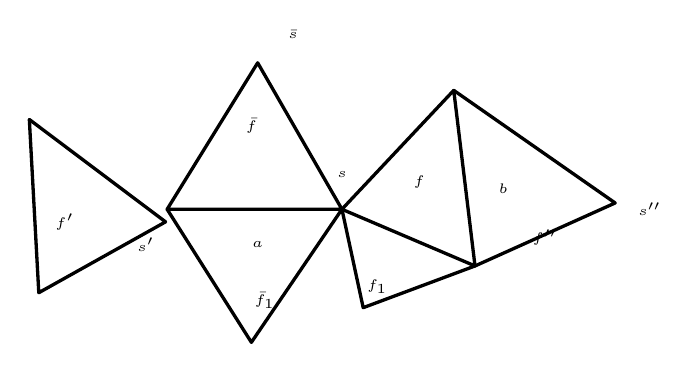
\begin{tikzpicture}[x=1mm,y=1mm,line cap=round,line join=round,font=\scriptsize]
\draw[very thick] (28,-36.4) -- (39.5,-17.8) -- (50.2,-36.4) -- cycle;
\draw[very thick] (28,-36.4) -- (38.7,-53.3) -- (50.2,-36.4);
\draw[very thick] (50.2,-36.4) -- (64.4,-21.3) -- (67.1,-43.6) -- cycle;
\draw[very thick] (64.4,-21.3) -- (84.9,-35.6) -- (67.1,-43.6);
\draw[very thick] (50.2,-36.4) -- (52.9,-48.9) -- (67.1,-43.6);
\draw[very thick] (10.5,-25) -- (11.7,-47) -- (27.8,-38) -- cycle;
\node[inner sep=1pt] at (44,-14.2) {\tiny $\bar s$};
\node[inner sep=1pt] at (38.7,-25.8) {\tiny $\bar f$};
\node[inner sep=1pt] at (39.5,-40.9) {\tiny $a$};
\node[inner sep=1pt] at (40.4,-48) {\tiny $\bar f_1$};
\node[inner sep=1pt] at (25.3,-40.9) {\tiny $s'$};
\node[inner sep=1pt] at (50.2,-32) {\tiny $s$};
\node[inner sep=1pt] at (60,-32.9) {\tiny $f$};
\node[inner sep=1pt] at (70.7,-33.8) {\tiny $b$};
\node[inner sep=1pt] at (76,-40) {\tiny $f''$};
\node[inner sep=1pt] at (89.3,-36.4) {\tiny $s''$};
\node[inner sep=1pt] at (54.7,-46.2) {\tiny $f_1$};
\node[inner sep=1pt] at (15,-38) {\tiny $f'$};
\end{tikzpicture}
\end{document}
